% !TeX spellcheck = en_US

\chapter{Extending solution DFAs to task DFAs} \label{ch:3}

Given a solution DFA $A_{sol}$ we have determined the following requirements for generating a task DFA $A_{task}$ in our requirements analysis (see~\ref{ch:1:determined-requirements}):
\begin{itemize}
	\item[->] $L(A_{sol}) = L(A_{task})$
	\item[->] $\mmD(A_{sol}) = \mmD(A_{task})$
	\item[->] number of duplicate states
	\item[->] number of unreachable states
	\item[->] alphabet size
	\item[->] planarity (can be checked in $O(|Q_{task}|)$)
	\item[->] completeness (for \MinMark-algorithm to work)
\end{itemize}
In order to fulfill these requirements when adding new elements to the given minimal automaton $A_{sol}$, we simply look at how duplicate and unreachable states are removed by the minimization algorithm, such that we can deduce from their properties, which restrictions are given for adding such elements. We will show for both classes of addable elements, that they do not change the DFAs language and its $\mmD$-value.

\gregor{Adding unreachable states is essentially just talking about that special equivalence class. Think and tell more about this}

\section{Adding duplicate states}

Firstly, let us state that since unreachable states are removed first in the minimization algorithm, we may assume that every state, that is duplicated, is reachable.

\gregor{hidden definition: correct duplication}
%\begin{definition}[Correct duplication]
%	Let $A = (Q, \Sigma, \delta, s, F)$ be the solution DFA and $A' = (Q', \Sigma, \delta', s, F')$ the task DFA with a $q_o, q_d \in Q'$, $q_d \notin Q$. Building such an $A'$ is called a \emph{correct duplication}, iff
%	\[
%		d_{A'}(q_o, q_d)
%	\]
%	and
%	\[
%		\forall q \in Q \colon [q]_{d_{A'}} = [q]_{d_A}
%	\]
%\end{definition}

Step 3 and 4 of the minimization algorithm are concerned with detection and elimination of duplicate states. How do we add duplicate states to a DFA?

Consider the properties a duplicate state, say $q_d$, must have. It is in particular duplicate to \emph{another} state, we call it $q_o$. We call the new, by $q_d$ extended DFA, $A$.

%  Since we add only one state for now, $q_d$, we can assume that $q_o$ is part of the solution DFA. 

\paragraph*{Outgoing transitions}

We know that $q_d$, $q_o$ are duplicates, iff $\forall \sigma \in \Sigma \colon [\delta(q_d, \sigma)]_{d_A} = [\delta(q_o, \sigma)]_{d_A}$. Thus, when adding some $q_d$, we have to choose for each symbol $\sigma \in \Sigma$ at least one transition from the following set:
\[
	P_\sigma = \{\ ((q_d, \sigma), p)\ |\ p \in [\delta(q_o, \sigma)]_{d_A}\ \}
\]
Since the solution DFA is complete, we know that every $P_\sigma \neq \emptyset$.

\gregor{Why does this not affect the eq. class of any other state?}

\paragraph*{Ingoing transitions}

The ingoing transitions of $q_d$ are not directly restricted through the duplicateness of $q_d$ and $q_o$.

First of all, we know, that $q_o$ is reachable. We then need to give $q_d$ at least one ingoing transition. Doing this, we have to ensure, that any state $s$, that gets such an outgoing transition to $q_d$ remains in its solution equivalence class.
	
Thus a fitting state $s$ has to have a transition to some state in $[q_d]_{d_A} = [q_o]_{d_A}$ already. So, given a state $s$ with $((s, \sigma), t)$ and $t \in [q_o]_{d_A}$, we can add $((s, \sigma), q_d)$.

But this would make our new DFA a NFA. As a consequence we have to remove the original transition $((s, \sigma), t)$ each time we add an ingoing transition for a newly created duplicate state.

So we have to choose at least one transition of
\[
	\{\ ((s, \sigma), q_d)\ |\ \delta(s,\sigma) \in [q_o]_{d_A}\ \}
\]
If a $((s, \sigma), q_d)$ is chosen, remove $((s, \sigma), t)$. This leads us to the requirement, that the equivalence class of any $q_o$ has to contain at least one state with at least $2$ ingoing transitions (see fig.~\ref{fig:dfa_add_duplicate_states}). We establish the following notion to pin down this restriction:
\[
	duplicatable(q_o) = 1 \Leftrightarrow_{def} (\exists q \in [q_o]_{d_A}\colon |d^-(q)| \geq 2)
\]
\begin{figure}
	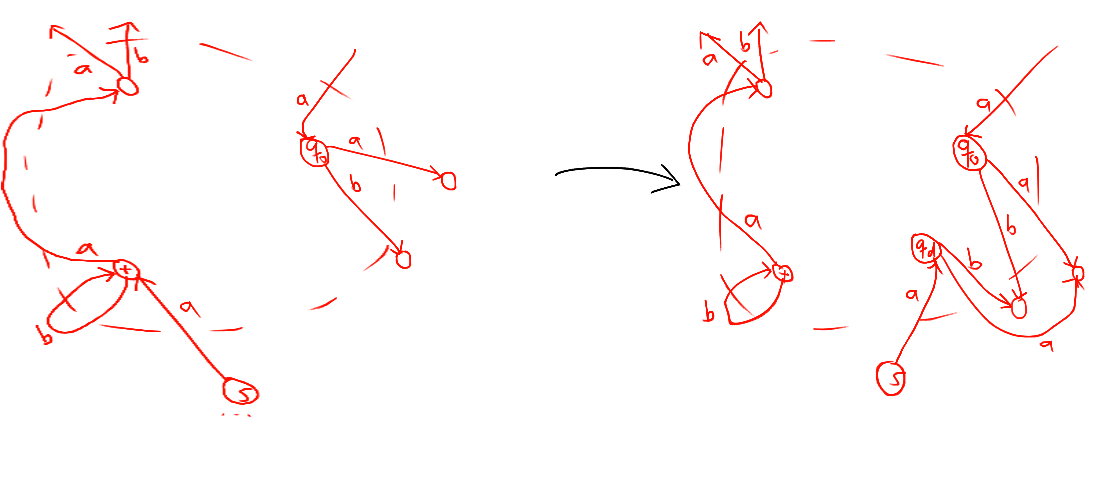
\includegraphics[width=\linewidth]{images/dfa_add_duplicate_states.png}
	\caption{If an equivalence class (here denoted by the states in the dashed area) contains a state with 2 or more ingoing transitions (in this case $t$), then a state duplicate to any of classes states may be added. Here $q_d$ is duplicate to $q_o$ and is ``stealing'' the ingoing transition $\delta(s, a)$ from $t$.}
	\label{fig:dfa_add_duplicate_states}
\end{figure}
\gregor{Talk somewhere about eq. automaton and extending it. An eq. class of reach. q's can be max. |$\Sigma$| big. From this can compute the max. number of dupl. states which can be added.}

\vspace{0.2cm}
\begin{algorithmic}[1]
	\Function{AddDuplicateStates\ }{$A_{sol}, d$}
	\State $eq\_classes \gets \{\ \{q\}\ |\ q \in Q\ \}$
	\State $eq\_class(q) = C$ such that $C \in eq\_classes$ and $q \in C$
	\State $\#_{d^-}(q) = |d^-(q)|$
	\State
	\For {$d$ \textbf{times}}
	
		\State
		\State $q_o \gets \bot$
		\For {$q$ \textbf{in} $C$}
			\If {$\#_{d^-}(q) \geq 2$}
				\State $q_0 \gets$ random chosen state from $eq\_class(q)$
				\State \textbf{break}
			\EndIf
		\EndFor
		\If {$q_o = \bot$}
			\State \Return $\bot$
		\EndIf
		
		\State
		\State $q_d \gets \max Q + 1$
		\State $Q \gets Q \cup \{ q_d \}$
		
		\State
		\For {$\sigma$ \textbf{in} $\Sigma$}
			\State $\delta(q_d, \sigma) =$ random chosen state from $eq\_class(\delta(q_o, \sigma))$
		\EndFor
		
		\State
		\State $O \gets \{\ ((s, \sigma), t) \in \delta\ |\ t \in eq\_class(q_o) \land \#_{d^-}(t) \geq 2\ \}$
		
		\State $C \gets$ random sample of at least one transition from $O$
		\For {$((s, \sigma), t)$ \textbf{in} $C$}
			\State $\delta \gets \delta \setminus \{((s, \sigma), t)\}$
			\State $\delta \gets \delta \cup \{((s, \sigma), q_d)\}$
			\State $\#_{d^-}(t) \gets \#_{d^-}(t) - 1$
			\State $\#_{d^-}(q_d) \gets \#_{d^-}(q_d) + 1$
		\EndFor
	\EndFor
	
	\State \Return $A$
	\EndFunction
\end{algorithmic}
\vspace{0.2cm}

\subsection{Adding duplicate states does not change L}

p. 159 Hopcroft

\subsection{Adding duplicate states does not change $\mmD$}

To prove this statement, we will prove two minor propositions first.

\begin{lemma}[Semantics of $(p,q) \in m(n)$] \label{ch:3:semantics-of-m(n)}
	\begin{multline*}
	(p,q) \in m(n) \Longleftrightarrow 
	\exists w\in\Sigma^*\colon |w| = n\ \land \\
	(\delta^*(p,w) \in F \Leftrightarrow \delta^*(q,w) \notin F)
	\end{multline*}
\end{lemma}

\begin{proof}
	See TI-Lecture ch. 4 ``Minimization'' p. 18.
\end{proof}

\begin{lemma}[Semantics of $\mmD(A) = n$] \label{ch:3:semantics-of-D(A)}
	\begin{multline*}
		\mmD(A) =\ n \Rightarrow \\
		n = \max_{n \in \mathbb{N}}\ \ \exists p, q \in Q\ \ \exists w \in \Sigma^* \colon |w| = n - 1\ \land \\
		(\delta^*(p,w) \in F \Leftrightarrow \delta^*(q,w) \notin F)
	\end{multline*}
\end{lemma}

\begin{proof}
	\begin{description}
		\item
		
		Via direct proof.
		
		Assume $m$-\MinMark(A) has done $n$ iterations (so $\mmD(A) = n$). We then know, that
		\begin{itemize}
			\item $\forall i \in [0,n-1]\colon m(i) \neq \emptyset$
			\item $m(n)= \emptyset$
		\end{itemize}
		$m$-\MinMark(A) terminates iff $m(i) = \emptyset$. If the first point would not hold, then the algorithm would have stopped before.
		
		Since the algorithm did $n$ iterations, the internal variable $i$ must be $n$ at the end of the last iteration. The terminating condition is $m(i) \neq \emptyset$; thus follows the second point.
		
		Recall the statement from lemma~\ref{ch:3:semantics-of-m(n)}:
		\begin{multline*}
		(p,q) \in m(n) \Longleftrightarrow 
		\exists w\in\Sigma^*\colon |w| = n\ \land \\
		(\delta^*(p,w) \in F \Leftrightarrow \delta^*(q,w) \notin F)
		\end{multline*}
	
		% a possible word per definition of D(A), m(i) and lemma
		
		Following this lemma and having $m(n-1) \neq \emptyset$ in mind, we can deduce that there exists at least one word $w\in\Sigma^*$ with $|w| = n-1$ such that for two $p,q \in Q\colon (\delta^*(p,w) \in F \land \delta^*(q,w) \notin F)$.
		
		% There is no word longer than that
		
		There cannot be any two states $p',q'\in Q$ and a word $w'\in\Sigma^*$ with $|w'| > n-1$ fulfilling this property. We could write $w'$ as $u'v'$ with $|v'| = n$. Then $m(n)$ would be non-empty, which is contradictory.
	\end{description}
\end{proof}

\begin{theorem}[]
	Adding duplicate states to an automaton $A$ does not increase the number of iterations in the \MinMark-algorithm for $A$.
\end{theorem}

\begin{proof}
	\begin{description}
		\item
		
		Proof per contradiction.
		
		Let's assume adding duplicate states $q_d^1, \ldots, q_d^n$ to a given automaton $A = (Q, \Sigma, \delta, s, F)$ results in an automaton $A' = (Q', \Sigma, \delta', s, F')$ whereas $\mmD(A) < \mmD(A')$.
		
		Concerning $A'$ we can say the following:
		\begin{itemize}
			\item $Q' = Q \cup \{ q_d^1, \ldots, q_d^n \}$
			%			\item $\delta \subseteq \delta'$
			%			\item $F \subseteq F'$
			\item W.l.o.g. $\exists q_o^1 \in Q \colon \exists q_o^2 \ldots q_o^n \in Q \colon\ d_A'(q_o^1, q_d^1), \ldots, d_A'(q_o^n, q_d^n)$
		\end{itemize}
		Let us furthermore say that $\mmD(A) = i$ and $\mmD(A') = j$. Recall now lemma~\ref{ch:3:semantics-of-D(A)}:
		\begin{multline*}
		\mmD(A) =\ n \Rightarrow \\
		n = \max_{n \in \mathbb{N}}\ \ \exists p, q \in Q\ \ \exists w \in \Sigma^* \colon |w| = n - 1\ \land \\
		(\delta^*(p,w) \in F \Leftrightarrow \delta^*(q,w) \notin F)
		\end{multline*}
		According to this lemma there must be a pair $s, t \in Q'$ to which exists a word $w \in \Sigma'^*$, $|w| = j - 1$, such that $\delta'^*(s,w) \in F' \Leftrightarrow \delta'^*(t,w) \notin F'$.
		
		Let us split $w$ as $w = uv$ such that $|v| = i$, which is exactly one symbol longer than the longest minimization word of $A$. We can formulate the following statement:
		\begin{equation}
		\text{There must exist }p, q \in Q'\text{ such that }\delta'^*(p,v) \in F' \Leftrightarrow \delta'^*(q,v) \notin F'.
		\end{equation}
		\gregor{hidden formulations here}
		%There must exist $p, q \in Q'$ such that $\delta'^*(p,v) \in F' \Leftrightarrow \delta'^*(q,v) \notin F'$.
		
		%So there exists a minimization word $v$ in $A'$, which is exactly one symbol longer than the longest minimization word of $A$. This word has length $i$ and is detected at minimization depth $i + 1$.
		
		We can therefore state, that $\neg(p \in Q \land q \in Q)$, because else $\mmD(A)$ would be higher than $i$ too.  So at least one of $p,q$ must be in $Q' \setminus Q$ which is exactly $\{ q_d^1, \ldots, q_d^n \}$.
		
		\begin{itemize}
			\item Every $q_d^k$ is $d_{A'}$-equivalent to a $q \in Q$
			\item In every case, $p,q$ can be $d_{A'}$-exchanged s.t. $p,q \in Q$
			\item But that's contradictory to $\mmD(A) = n$, because $p,q$ belong to a minimization word $w = n-1$
		\end{itemize}
		
%		Since $q_d$ is the only new state in $A'$ compared to $A$, we can conclude that at least one of both states must be $q_d$. Since $p = q_d = q$ is contradictory (\gregor{why?}), we can conclude that exactly one of both states $p, q$ is $q_d$ and that the other one is not.
%		
%		W.l.o.g.\ we say $q = q_d$ and $p \in Q' \setminus \{q_d\} = Q$ and reformulate our statement above:
%		\begin{equation}
%		\text{There must exist a }p \in Q\text{ such that }\delta'^*(p,v) \in F' \Leftrightarrow \delta'^*(q_d,v) \notin F'.
%		\end{equation}
%		\gregor{hidden formulations here}
%		
%		%Therefore we know there exists a state $p \in Q$ such that $\exists v \in \Sigma^*$, $|v| = i$ and $\delta'^*(p,v) \in F' \Leftrightarrow \delta'^*(q_d,v) \notin F'$
%		
%		Since for $q_o \in Q$ the relation $d_{A'}(q_o, q_d)$ is given, we know per definition of $d_{A'}$ that $\forall z\in\Sigma'^*\colon \delta'^*(q_o,z) \in F \Leftrightarrow \delta'^*(q_d,z) \in F$.
%		
%		This implies in combination with statement 2.2, that for $p,q_o$ the word $v\in\Sigma'^*$ would fulfill $\delta'^*(p,v) \in F' \Leftrightarrow \delta'^*(q_o,v) \notin F'$ too. But this is contradictory to $p,q \notin Q$.
	\end{description}
\end{proof}

\gregor{Old proof for one $q_d$}
%\begin{proof}
%	\begin{description}
%		\item
%		
%		Proof per contradiction.
%		
%		Let's assume adding a duplicate state $q_d$ to a given automaton $A = (Q, \Sigma, \delta, s, F)$ results in an automaton $A' = (Q', \Sigma, \delta', s, F')$ whereas $\mmD(A) < \mmD(A')$.
%		
%		Concerning $A'$ we can say the following:
%		\begin{itemize}
%			\item $Q' = Q \cup \{ q_d \}$
%			%			\item $\delta \subseteq \delta'$
%			%			\item $F \subseteq F'$
%			\item $\exists q_o \in Q \colon\ d_A'(q_o, q_d)$
%		\end{itemize}
%		Let us furthermore say that $\mmD(A) = i$ and $\mmD(A') = j$. Recall now lemma~\ref{ch:3:semantics-of-D(A)}:
%		\begin{multline*}
%			\mmD(A) =\ n \Rightarrow \\
%			n = \max_{n \in \mathbb{N}}\ \ \exists p, q \in Q\ \ \exists w \in \Sigma^* \colon |w| = n - 1\ \land \\
%			(\delta^*(p,w) \in F \Leftrightarrow \delta^*(q,w) \notin F)
%		\end{multline*}
%		According to this lemma there must be a pair $s, t \in Q'$ to which exists a word $w \in \Sigma'^*$, $|w| = j - 1$, such that $\delta'^*(s,w) \in F' \Leftrightarrow \delta'^*(t,w) \notin F'$.
%		
%		Let us split $w$ as $w = uv$, whereas $u,v \in\Sigma'^*$ and $|v| = i$, which is exactly one symbol longer than the longest minimization word of $A$. We can formulate the following statement:
%		\begin{equation}
%		\text{There must exist }p, q \in Q'\text{ such that }\delta'^*(p,v) \in F' \Leftrightarrow \delta'^*(q,v) \notin F'.
%		\end{equation}
%		\gregor{hidden formulations here}
%		%There must exist $p, q \in Q'$ such that $\delta'^*(p,v) \in F' \Leftrightarrow \delta'^*(q,v) \notin F'$.
%		
%		%So there exists a minimization word $v$ in $A'$, which is exactly one symbol longer than the longest minimization word of $A$. This word has length $i$ and is detected at minimization depth $i + 1$.
%		
%		We can therefore state, that $\neg(p \in Q \land q \in Q)$, because else $\mmD(A)$ would be higher than $i$ too. 
%		
%		Since $q_d$ is the only new state in $A'$ compared to $A$, we can conclude that at least one of both states must be $q_d$. Since $p = q_d = q$ is contradictory (\gregor{why?}), we can conclude that exactly one of both states $p, q$ is $q_d$ and that the other one is not.
%		
%		W.l.o.g.\ we say $q = q_d$ and $p \in Q' \setminus \{q_d\} = Q$ and reformulate our statement above:
%		\begin{equation}
%		\text{There must exist a }p \in Q\text{ such that }\delta'^*(p,v) \in F' \Leftrightarrow \delta'^*(q_d,v) \notin F'.
%		\end{equation}
%		\gregor{hidden formulations here}
%		
%		%Therefore we know there exists a state $p \in Q$ such that $\exists v \in \Sigma^*$, $|v| = i$ and $\delta'^*(p,v) \in F' \Leftrightarrow \delta'^*(q_d,v) \notin F'$
%		
%		Since for $q_o \in Q$ the relation $d_{A'}(q_o, q_d)$ is given, we know per definition of $d_{A'}$ that $\forall z\in\Sigma'^*\colon \delta'^*(q_o,z) \in F \Leftrightarrow \delta'^*(q_d,z) \in F$.
%		
%		This implies in combination with statement 2.2, that for $p,q_o$ the word $v\in\Sigma'^*$ would fulfill $\delta'^*(p,v) \in F' \Leftrightarrow \delta'^*(q_o,v) \notin F'$ too. But this is contradictory to $p,q \notin Q$.
%		
%		\gregor{hidden lemma here}
%		
%		%		\begin{lemma}
%		%			\begin{multline*}
%		%				\mmD(A) =\ n \Leftrightarrow \\
%		%				n = \max_{n \in \mathbb{N}}\ \ \exists p, q \in Q\ \ \exists w \in \Sigma^* \colon \\
%		%				|w| = n - 1 \land (\delta^*(p,w) \in F \Leftrightarrow \delta^*(q,w) \notin F)
%		%			\end{multline*}
%		%		\end{lemma}
%	\end{description}
%\end{proof}


\gregor{hidden old 'systematic study of how to extend minimal DFAs'}
%First, a systematic study of how to extend minimal DFAs will be done. Afterwards, we will define an extension algorithm, which will use the previously found results. We have the following requirements for this stage:
%\begin{itemize}
%	\item the language of the task DFA is the same as the language of the solution DFA
%	\item $\mmD(A_{sol}) = \mmD(A_{task})$
%	\item the number of new elements should be controllable
%\end{itemize}
%
%\section{Adding new elements to DFAs}
%
%Our study of DFA extension possibilities will focus on methods, that add or remove transitions or states. A solution DFA modified by such methods will be denoted as $A_{sol'}$. In general, we could also change start and accepting nodes, but we will exclude these possibilities here. As a consequence, we may now classify our options as follows:
%\begin{enumerate}
%	\item Add states and no transitions
%	\item Add transitions and no states
%	\item Add states and transitions such that
%	\begin{itemize}
%		\item At least one state is added
%		\item No new state has no transitions
%	\end{itemize}
%	\item Remove/add states and transitions such that
%	\begin{itemize}
%		\item At least one state or transition is removed
%	\end{itemize}
%\end{enumerate}
%Adding states $p_1, \ldots, p_n$ and no transitions leads to the situation, that $p_1, \ldots, p_n$ are lonely states. Since adding lonely states does not affect an automatons language, we can use this as option to extend DFAs.
%
%Adding new transitions does not work because of minimal automaton isomorphism \ldots
%
%For option 3, we can not tell yet, whether it will generate usable automatons. The two additional conditions guarantee, that the generated automatons are distinct from the ones generated by options 1 and 2 \\
%
%\noindent One could imagine, that removing transitions/states and adding new ones again might generate distinct automatons in relation to option 3. However, we can prove, that each automaton generated by this technique is isomorphic to an automaton generated by option 3.
%
%\begin{proof}
%	To a given language $L$ only one minimal automaton $A_L$ (despite isomorphism) exists.
%	So every "remove-add"-automaton $A_{ra}$ can be transformed to $A_L$ using the minimization algorithm.
%	The minimization algorithm does in particular delete some states and transitions.
%	Thus adding these states and transitions to $A_L$ is the way to simulate the generation via "remove-add" through generation via "just-add".
%\end{proof}
%\noindent As a consequence, we will discuss from now on only option 3 in more detail.
%
%\section{Add states and transitions}
%
%We classify several subcases:
%
%\begin{enumerate}
%	\item New states have ingoing transitions only
%	\begin{enumerate}
%		\item All new states are non-accepting
%		\item At least one state is accepting
%	\end{enumerate}
%	\item New states have outgoing transitions only
%	\item New states have both in- and outgoing transitions
%\end{enumerate}
%Adding states $p_0, \ldots, p_n$ with ingoing transitions is okay, if there is a sink-state in $A_{sol}$ and if every $p_i$ is non-accepting and thus a sink-state.
%
%We prove that adding accepting states with ingoing transitions only leads to a NFA or to a DFA with a different language.
%\begin{proof}
%	If a new state $p$ is accepting and if w.l.o.g.\ $\delta(q, \sigma) = p$, then there are several cases:
%	\begin{itemize}
%		\item $p$ is unreachable: Then we got at least one unreachable sub-graph consisting of more than one states
%		\item $p$ is reachable: Then the language of the solution automaton (call it $A_{sol}$) is not preserved. This is because of the following:
%		
%		If $A_{sol}$ were in state $q$ after reading $w \in \Sigma^*$ with $\sigma$ as next Symbol, then there would have to exist a transition $\delta(q, \sigma) = p'$ whereas $p' \in F$ is an accepting state. But this would imply that $A_{sol}$ is an NFA (contradiction).
%	\end{itemize}
%\end{proof}
%
%\noindent 2. leads to the new state being unreachable.
%
%Thus we remain with option 3, which states that every new state has at least one ingoing transition and at least one outgoing transition.
%
%\section{New states have both in- and outgoing transitions}




%\subsection{Usable results}

%1. Add states only -> unreachable and sink-state \\
%2. Add transitions only -> does not increase state number \\
%3. Add/Remove states and transitions -> generated by 4. too \\
%4.1. Adding states with ingoing transitions only -> sink-states, NFA or different lang. \\
%4.2. Adding states with outgoing transitions only -> unreachable \\
%4.3.1. Adding states and duplicate at least its ingoing transitions -> NFA \\
%4.3.2. Adding states, split ingoing, duplicate outgoing -> generated by 4.3.2.1. too \\
%4.3.2.1. Adding states, split ingoing, split outgoing s.t. $[\delta(q', \sigma_i)]_{\equiv_L} = [\delta(q'', \sigma_i)]_{\equiv_L}$ -> Ok

\section{Adding unreachable states}

From step 1 of the minimization algorithm we can deduce how to add unreachable states. These can easily be added to a DFA by adding non-start states with no ingoing transitions (see def.~\ref{ch:1:unreachable-states}). Number and nature of outgoing transitions may be arbitrary.

\vspace{0.2cm}
\begin{algorithmic}[1]
	\Function{AddUnreachableStates\ }{$A, u$}
	\For {$u$ \textbf{times}}
		\State $q \gets \max Q + 1$
		\State $Q \gets Q \cup \{ q \}$
		\State $R \gets$ random chosen sample of $|\Sigma|$ states from $Q \setminus \{q\}$
		\For {$\sigma$ \textbf{in} $\Sigma$}
			\State $q' \in R$
			\State $R \gets R \setminus \{q'\}$
			\State $\delta \gets \delta \cup \{ ((q, \sigma), q') \}$
		\EndFor
	\EndFor
	\State \Return $A$
	\EndFunction
\end{algorithmic}
\vspace{0.2cm}

\noindent We have to ensure, that this algorithm does not induce changes in the language.
\begin{lemma}
	Adding unreachable states to a DFA does not change its language.
\end{lemma}
\begin{proof}
	Remember that the language of a DFA $A = (Q, \Sigma, \delta, s, F)$ is defined as $L(A) = \{\ w\ |\ w \in \Sigma^* \ \}$. For any unreachable state $q$ there exists no word $v \in \Sigma^*$ such that $\delta^*(s,v) = q$. Thus such a state cannot be the cause for any word to be in $L(A)$.
\end{proof}

\noindent The question whether adding unreachable states to a DFA changes $\mmD$-value is irrelevant. This is because in the context of the minimization algorithm, unreachable states are eliminated before the \MinMark-algorithm is applied on the task DFA.
